\chapter{Diseño}

{\color{blue}


Se van a mostrar las tecnologías usadas en el proyecto, así como las decisiones tomadas a la hora del desarrollo del software. En este proyecto, tenemos por un lado nuestra aplicación, la cual va a recoger todos los datos y por otro lado tenemos un dispositivo, que este es una Raspberry PI \cite{raspberry-specs}, prestada por mis tutores de proyecto. Para hacer la conexión entre aplicación y dispositivo se necesita hacer uso de un protocolo de mensajería, en este caso se opta por el uso de MQTT. \\

También se va a mostrar como se va a proceder para la explotación de la vulnerabilidad y cuestiones a tener en cuenta.

\section{Tecnologías usadas en la creación de la aplicación}

\subsection{Lenguaje de programación}

Se ha optado por usar Python, fue creado a principios de los años 90 por Guido van Rossum en el Stichting Mathematisch Centrum en los Países Bajos como sucesor de un lenguaje llamado ABC. Guido sigue siendo el principal autor de Python, aunque incluye muchas contribuciones de otras personas. \\

En mayo de 2000, Guido y el equipo de desarrollo del núcleo de Python se trasladaron a BeOpen.com para formar el equipo BeOpen PythonLabs. En octubre del mismo año, el equipo de PythonLabs se trasladó a Digital Creations. En 2001, se formó la Python Software Foundation, una organización sin ánimo de lucro creada específicamente para poseer la propiedad intelectual relacionada con Python. \cite{python-history} \\

Python es un lenguaje de alto nivel de programación interpretado cuya filosofía hace hincapié en la legibilidad de su código, se utiliza para desarrollar aplicaciones de todo tipo. Se trata de un lenguaje de programación multiparadigma, ya que soporta parcialmente la orientación a objetos, programación imperativa y, en menor medida, programación funcional. Es un lenguaje interpretado, dinámico y multiplataforma. \cite{python-wiki} \\

Para este proyecto es una buena opción ya que gracias a paquetes como \textbf{paho-mqtt}, que proporciona una clase cliente que permite a las aplicaciones conectarse a un broker MQTT para publicar mensajes, y para suscribirse a temas y recibir mensajes publicados, podemos hacer conexiones a mqtt de una manera muy sencilla. \cite{paho-mqtt}

\subsection{Pycharm}

PyCharm es un entorno de desarrollo integrado utilizado en programación informática, concretamente para el lenguaje de programación Python. Está desarrollado por la empresa checa JetBrains. Proporciona análisis de código, un depurador gráfico, un probador de unidades integrado, integración con sistemas de control de versiones (VCS), y soporta el desarrollo web con Django, así como la ciencia de datos con Anaconda. \\

PyCharm es multiplataforma, con versiones para Windows, macOS y Linux. La Community Edition (edición comunitaria) se publica bajo la Licencia apache, y también hay una Professional Edition (edición profesional) con características adicionales publicada bajo una licencia propietaria financiada por suscripción y también una versión educativa, que gracias a la universidad de Granada podemos hacer uso de esta licencia. \cite{pycharm}

\subsection{Diagrama de clases}

Para hacer la comunicación entre el dispositivo y la aplicación se propone el siguiente diagrama de clases que describe la estructura del sistema. 

\begin{figure}[p]
    \centering
    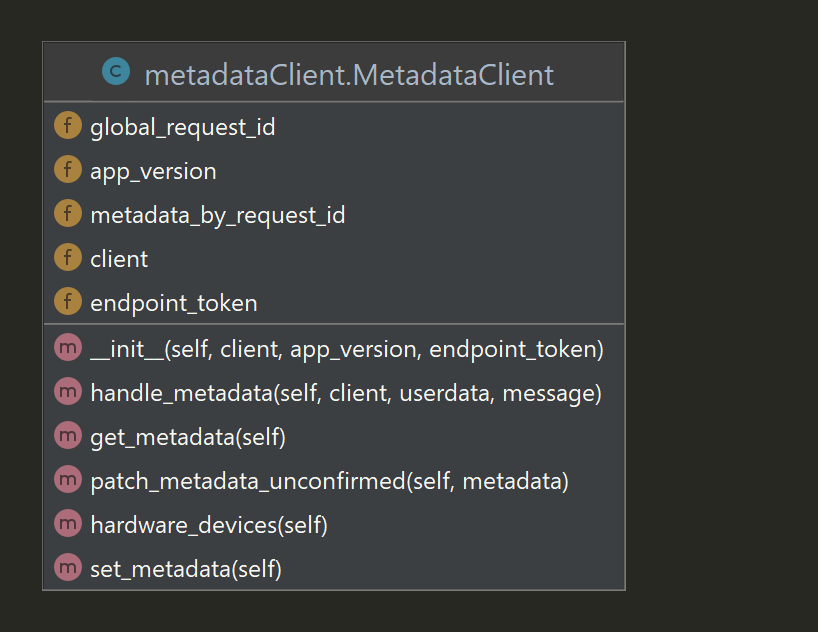
\includegraphics[width=\linewidth]{imagenes/metadataClient.png}
    \caption{Clase de envio de metadatos del dispositivo}
    \label{fig:figure-diseño1}
\end{figure}

\begin{figure}[p]
    \centering
    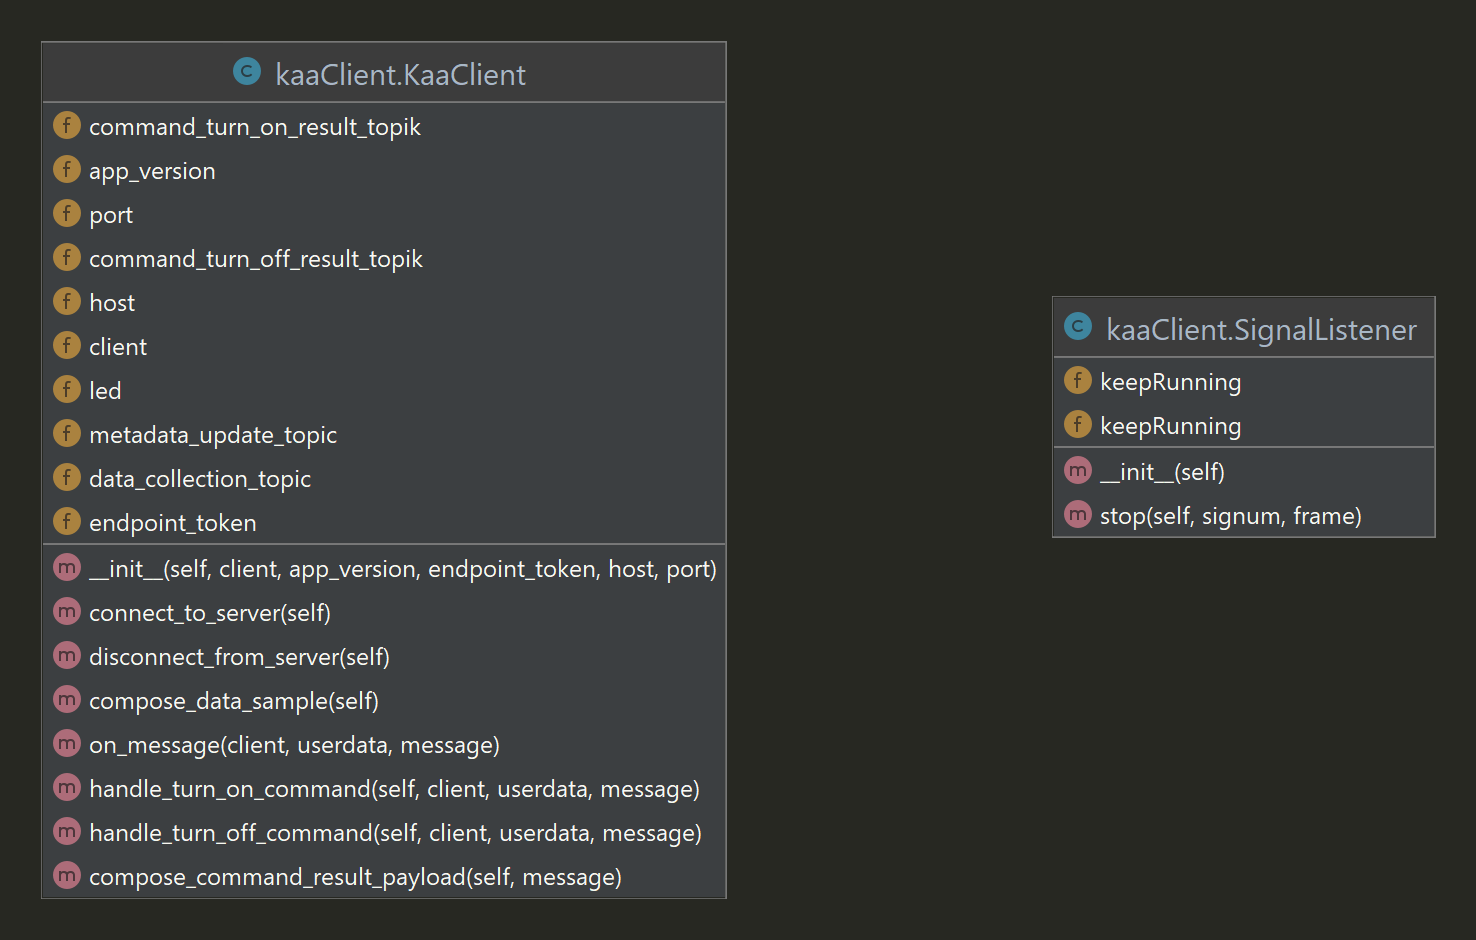
\includegraphics[width=\linewidth]{imagenes/kaaClient.png}
    \caption{Clase de envio de datos de telemetría y ejecución de comandos}
    \label{fig:figure-diseño2}
\end{figure}

La clase \textit{MetadataClient} \ref{fig:figure-diseño1} establece una primera conexión con la aplicación, recoge los datos a nivel hardware de la Raspberry y los envía para actualizar la información en la aplicación. \\

La segunda clase \textit{KaaClient}, hace una conexión con la cual enviamos datos de telemetría, en concreto, obtenemos cada cierto tiempo la temperatura de la CPU de la Raspberry y se envía esta y el momento de tiempo en el que se produce el envio. También incluye funciones para gestionar el encencido y apagado de un led conectado a la Raspberry. \\

El led estará conectado a la Raspberry como se muestra en la figura \ref{fig:figure12}.

\begin{figure}[p]
    \centering
    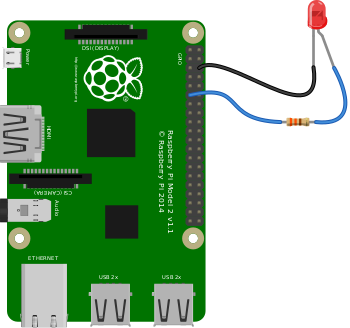
\includegraphics[width=\linewidth]{imagenes/led_bb.png}
    \caption{Conexion del led con Raspberry \cite{raspberry-led}}
    \label{fig:figure12}
\end{figure}

Por último, la clase \textbf{SignalListener} que se usa para poder parar la ejecución de la comunicación desde una E/S. \\

\subsection{Bibliotecas usadas}

\subsubsection{subprocess}

Para obtener los dispositivos conectados a la Raspeberry se usa \textbf{subprocess}. El módulo de subprocesos permite generar nuevos procesos, conectarse a sus tuberías de entrada/salida/error y obtener sus códigos de retorno. \cite{subprocess}

\subsubsection{GPIO Zero}

Una sencilla interfaz para dispositivos GPIO con Raspberry Pi, desarrollada y mantenida por Ben Nuttall y Dave Jones. Se usa para obtener la temperatura de la CPU y para encender/apagar el led de la Raspberry. \cite{gpiozero}

\subsubsection{decouple}

Decouple ayuda a organizar la configuración para que puedas cambiar los parámetros sin tener que volver a desplegar la aplicación. En un fichero .env se almacena los datos sensibles para no mostrarlos al público y se cargan una vez antes de iniciar la comunicación. \cite{decouple}

\subsubsection{paho mqtt}

Como se ha mencionado ya, sirve para establecer la conexión mqtt. \cite{paho-mqtt}


}